
\documentclass[paper=a4]{scrartcl}

\usepackage[left=4cm, right=4cm
  %,showframe% <- only to show the page layout
]{geometry}

\addtolength{\parskip}{\baselineskip} 
\parindent 0pt

\usepackage{graphicx}
\usepackage{config}

\begin{document}

\begin{center}
{\Large{\textbf{ Non-random network connectivity comes in pairs }}}

%(connection probablities that are symmetric in pairs)
\end{center}
\centerline{}
\centerline{Felix Z.~Hoffmann, Jochen Triesch}

\vspace{1cm}

Overrepresentation of bidirectional connections in local cortical networks has been repeatedly reported and is in the focus of the ongoing discussion of non-random connectivity. Here we show in a brief mathematical analysis that in a network in which connection probabilities are symmetric in pairs, $P_{ij} = P_{ji}$, the occurrence of bidirectional connections and non-random structures are inherently linked; an overabundance of reciprocally connected pairs emerges necessarily when the network structure deviates from a random network in any form. For two distributions of connection probabilities, the discrete two-point distribution and continuous gamma distribution, we quantify how a more organized structure increases reciprocity in the network.


\vspace{1cm}

\begin{figure}[h!]
  \centering
  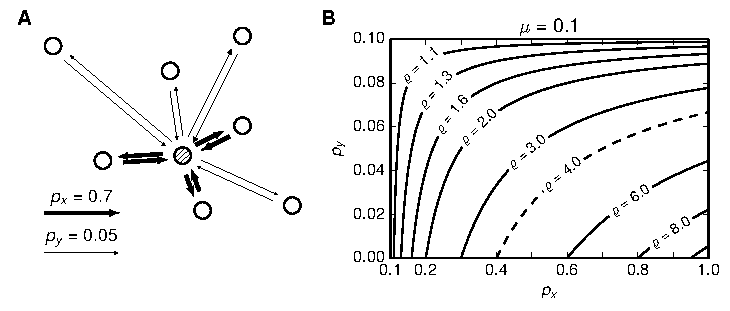
\includegraphics[width=\textwidth]{%
    ../figures/two_point_full/pub/two_point_full_pxpy.pdf} %
\end{figure}

\nocite{Song2005, Perin2011}

\printbibliography

\end{document}
